\documentclass{article}

\usepackage[french]{babel}
\usepackage[utf8]{inputenc}
%\usepackage{lmodern}
\usepackage[T1]{fontenc}
\usepackage{hyperref}
\usepackage{times}
\usepackage{graphicx}
\usepackage{csquotes}
\usepackage{amssymb}
\usepackage{fancyhdr}


\pagestyle{fancy}
\renewcommand\headrulewidth{0.5pt}
\fancyhead[L]{\LaTeX \quad Pavage et pavabilité dans le plan}
\fancyhead[R]{Université de Bordeaux}



\title{Pavages et pavabilité dans le plan}
\author{A. HIPPOLYTE, R. CHAVAGNAC, M. DE MURET DE LABOURET}

\begin{document}

\maketitle

\tableofcontents

\newpage

\section{Introduction}

\subsection{Pavage du plan}

Un pavage P dans un plan est un ensemble fini d'éléments compacts et d’interieur non vide.
P a une frontière F (points au contact de P et de son complementaire(ensemble des elements de E qui n'appartienent pas à P)) et un intérieur (emsemble des points de P qui n'appartiennent pas à F).
On dit que P est fermé si F appartient à P.
Un pavage est une partition du plan (euclidien, hyperbolique \footnote{ espace qui ne vérifie pas le 5eme postulat d’Euclide (si un point P est extérieur à une droite d1, il n’existe qu’une droite d2 parallèle à d1 qui passe par P). Il existe une infinité de droites différentes parallèle à une même droite. }…).

On peut aussi paver dans un espace de dimension supérieur au plan mais nous allons nous concentrer sur l’espace à deux dimensions.
Chaque élément de P possède au moins un côté connexe a un autre.
Il peut y avoir plusieurs éléments de forme différentes pour paver un plan.

\subsection{Pavage régulier}

Lorsque les même éléments sont représentés plusieurs fois, on dit que le pavage est regulier (irrégulier si non).
Les sous-espaces de P sont image l’un de l’autre par une isométrie du plan \footnote{ Soit E un espace vectoriel euclidien. Une application linéaire f dans E est appelée isométrie linéaire ssi , quel que soit l’élément m de E , on a $\left \| f\left ( m \right ) \right \| = \left \| m \right \|$ , autrement dit, ssi f conserve la norme dans E transformation bijective d'un espace dans un autre (dans le plan : translation, rotation, symetrie centrale, symétrie axiale, symétrie glissée)}.
Pour tout couple $\left ( p_{1} ,p_{2}\right )$ d'élément de P régulier, il existe une isometrie du pavage f tel que $f\left (  p_{1}\right )=p_{2}$.

\begin{figure} [h]
    \center
    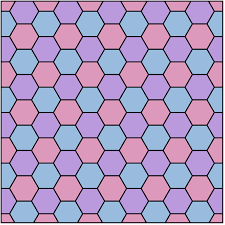
\includegraphics [scale=0.5] {image/pavage_hexagonal.png}
    \caption{Exemple de pavage régulier avec des hexagones}
\end{figure}

\newpage

\subsection{Pavage périodique / aperiodique}

\hspace{1.5cm}

\textbf{\textsc{Périodique}}

Un pavage P est périodique s'il est composé d'elements répétés sur une portion regulière du plan.
On peut le retrouver sur les murs du palais de l'Alhambra ou sur les dessins de M.C Escher (pavage hyperbolique).
Ce type de pavage est connu depuis l’antiquité comme motif décoratif.

\begin{figure} [h]
    \center
    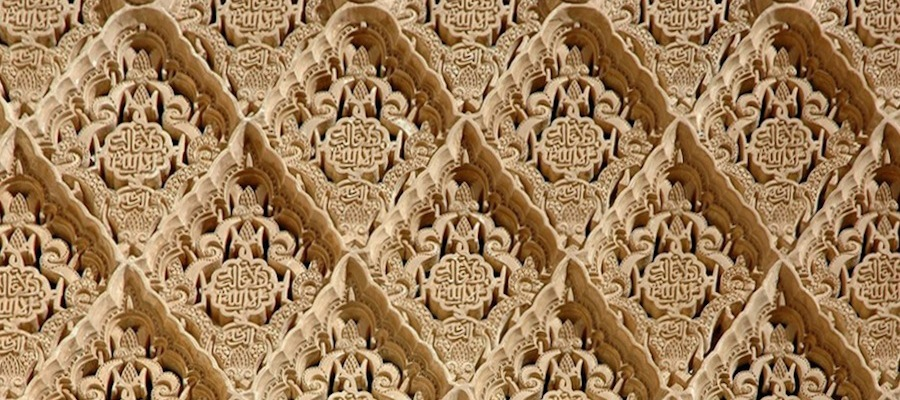
\includegraphics [scale=0.3] {image/Alhambra.jpg}
    \caption{Portion de mur de l'Alhambra}
\end{figure}

Le mathematicien russe Fedorov a montré que seulement 17 types de pavages periodiques existaient dans le plan.
Deux pavages sont considérés de meme type s’ils sont invariant par le meme groupe d’isométrie.
On retrouve les 17 types de pavages à l'Alhambra.

\begin{figure} [h]
    \center
    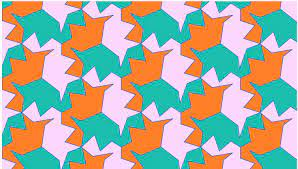
\includegraphics [scale=0.5] {image/Ex1_pavage.jpg}
    %\caption{Diamants aztèques d'ordre 1, 2, 3 et 6}
\end{figure}

\hspace{1.5cm}

\textbf{\textsc{Apériodique}}

Un pavage est apériodique s'il est composé d'ensemble d'élements répétés apériodiquement.

Un puzzle est un pavage apériodique la forme est unique pour chaque piece et les couleurs ne représentent pas de motifs périodiques.


Le pavage de Penrose est l'exemple le plus connu.
Ce type de pavage répond à plusieurs règles précises.

\newpage

Il existe 4 pavages de Penrose différents :

\hspace{1cm}

- Pentagonal ( avec des pentagones, losanges, pentagrammes et des portions de pentagramme).

\begin{figure} [h]
    \center
    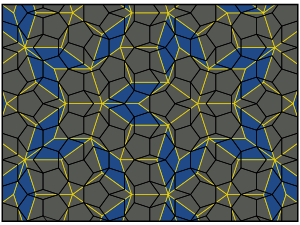
\includegraphics [scale=0.4] {image/penrose_pentagone.png}
    \caption{Pavage de Penrose pentagonal tracé en noir}
\end{figure}

\hspace{1.5cm}

- Cerfs-volant et fléchettes ( avec deux quadrilatères, l'un convexe, l'autre concave )

\begin{figure} [h]
    \center
    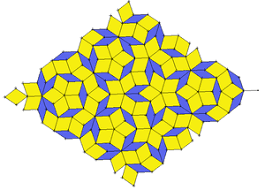
\includegraphics [scale=0.5] {image/penrose_flechette.png}
    \caption{Pavage de Penrose en fléchettes}
\end{figure}

- Losanges ( avec deux sortes de losanges, fins et gros )

\begin{figure} [h]
    \center
    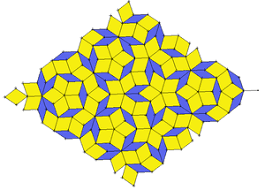
\includegraphics [scale=0.5] {image/penrose_losange.png}
    \caption{Pavage de Penrose avec des losanges}
\end{figure}

- Triangle d’or ( avec des triangles isocèles dont les cotés ont des longueurs proportionnelles au nombre d’or )

\begin{figure} [h]
    \center
    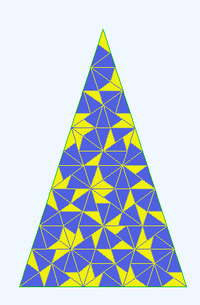
\includegraphics [scale=0.5] {image/penrose_tri.png}
    \caption{Pavage de Penrose avec de triangles d'or}
\end{figure}

\newpage

\section{Pavage du plan par des dominos}

Aucun algorithme ne dit systématiquement si une portion de plan est pavable par des polygones.
On dit que le problème est indécidable \footnote{Problème qui ne peut pas être résolu algorithmiquement en un temps toujours fini.}.

Dans cette partie, nous allons alors nous concentrer sur le pavage par dominos, le domino $2*1$ et $1*2$.
Soit P le pavage construit par les dominos dans . P est une portion finie de plan délimitée par des côtés de longueur entière parallèles aux axes du plan euclidien.
On considere aussi que ce sous espace de $\mathbb{Z}^{2}$ n’a pas de trous. Ce type de pavage est régulier par isométrie du plan et apériodique.
Les dominos ne doivent pas se chevaucher et sont connexes à au moins un autre domino.

\begin{figure} [h]
    \center
    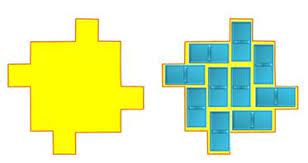
\includegraphics [scale=0.5] {image/pavage_domino.jpg}
    \caption{Exemple d'un pavage possible d'une portion du plan par des dominos }
\end{figure}

\clearpage

\subsection{Polyomino}

Un polyomino est une réunion connexe et finis de carrés unitaires de $\mathbb{Z}^{2}$ (ex: formes de Tetris) chaque carré a au moins un coté connexe a un autre.
Il existe 2 groupes de polyomino : à forme fixée et à forme libre (qui peut subir une rotation ).

\begin{figure} [!h]
    \center
    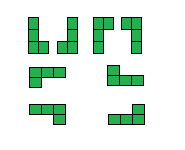
\includegraphics [scale=0.5] {image/polyomino_libre.png}
    \caption{8 formes fixes pour une même forme libre d'un tétromino (4 carrés)}
\end{figure}

\hspace{1cm}

Un domino est un polyomino appartenant à $\mathbb{Z}^{2}$ composé de 2 carrés. Il n’a qu’une forme libre possible et deux formes fixées : $2*1$ et $1*2$.
Un triomino est composé de 3 carrés et a deux formes libres possibles.

\hspace{1cm}

\begin{figure} [!h]
    \center
    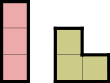
\includegraphics [scale=0.5] {image/triomino.png}
    \caption{Les deux formes libres du triomino}
\end{figure}

\hspace{1cm}

Ainsi de suite, un decamino (10 carrés) a 4655 formes libres différentes.

Un pavage dans $\mathbb{Z}^{2}$ est un polyomino composé de sous-polyominos (ici les dominos).
Etant donné un ensemble finis P de polyomino, la pavabilité est decidable puisqu'on peut toujours essayer toutes les combinaisons possibles.
Il s'agit alors de trouver un algorithme efficace pour dire si un polyomino est pavable ou non par des dominos.

\newpage

\subsection{Algorithme de Thurston}

L'algorithme de Thurston décide en temps linéaire si un polyomino sans trou est pavable par dominos et le construit si oui.
Prenons un polyomino de n cases, sa complexité est en $O\left ( nlog\left ( n \right ) \right )$. Soit p son périmetre, p=racine de n car n est son air.
Ainsi on peut aussi dire que sa complexité est en $O\left ( p^{2}log\left ( p^{2} \right ) \right )$.

Considérons un polyomino sans trou. On colorie ses cases comme un damier (cadrié en noir et blanc). Ce polyomino peut etre représenté par un graphe dont les arretes seraient les cotés des cases du damier.
On definit une fonction de hauteur h appliqué aux n sommets du graphe G {v0,v1,...,vn}.
Partons d'un sommet v0 quelconque.

- $h\left ( v_{0} \right )= 0$

Soient vi et vj deux sommets de G reliés par une arrete alors

- $h\left ( v_{j} \right )= h\left ( v_{i} \right ) + 1$ si l'arrete (vi,vj) a sur sa gauche une case noire.

- $h\left ( v_{j} \right )= h\left ( v_{i} \right ) - 1$ si non.




\newpage

\subsection{Nombre de pavage dans un polyomino}

\hspace{1cm}

\subsubsection{Nombre de pavage dans un rectangle mxn}

\hspace{1.5cm}

\textbf{\textsc{2xn}}

Soit $f_{n}$ le nombre de pavage possible.

Le premier cas est le rectangle $2*1$, il y a bien sûr qu’un pavage possible : $f_{1} = 1$.

Le deuxieme cas est un rectangle $2*2$, où deux pavages sont possibles deux dominos en long ou deux dominos en large.

\begin{figure} [!h]
    \center
    \includegraphics [scale=0.5] {image/pavage_carré.png}
    \caption{Les deux facons de paver un carré  $2*2$}
\end{figure}

Dans un cas général, si on ajoute au rectangle $2*n$ un rectangle sur le coté de longueur 2, le nombre $f_{n}$ de pavage augmente de 1.

Mais on peut aussi ajouter deux rectangles en long au rectangle $2*(n+1)$ sur le coté de longueur 2. Dans ce cas là, le nombre $f_{n-1}$ de pavage augmente de 2.

Ainsi on a tous les pavages du rectangle $2*(n+1)$ et $f_{n+1} = f_{n} + f_{n-1}$.

Ce sont les nombres de Fibonacci : 1, 2, 3, 5, 8, 13, 21, 34, 55…

Le rectangle de dimension $2*10$ a 89 pavages possibles.

\hspace{1.5cm}

\textbf{\textsc{3x2n}}

Bien sur un rectangle de dimension $3*(2n+1)$ est impossible à paver puisqu'il y a un nombre impair de cases.

Le premier cas est un rectangle $3*2$, il y a trois pavages possibles (image), $f_{3} = 3$.

Si on y ajoute un deuxieme blos $3*2$, il y a $3*3$ pavages possibles dans chaque bloc.
Mais on peut aussi former 2 pavages dans le rectangle $3*4$ sans former de bloc $3*2$.

Ainsi, en général, si on appelle $a_{n}$ le nombre de pavage dans un rectangle de $3*2n$, $a_{n+1}$ est obtenu en y ajoutant un bloc de 3×2.
Ce qui donne $3*a_{n}$, plus toutes les combinaisons où ce bloc est concaténé avec des blocs précédents sans former de blocs de 3×2.
Dans ce cas, il y a un bloc de $3*2i$ suivi d'un bloc de $3*2j$ sans blocs internes. Il n'y a que deux possibilités obtenues en dupliquant les dominos rouges de l'exemple $3*4$. (image)

Chacune de ces possibilités donne donc lieu à $a_{i}*2$ possibilités.

Donc $a_{n+1} = 3*a_{n} + 2\sum_{i}^{n}a_{i}$

Calculons $a_{n+1} - a_{n}$

$a_{n+1} - a_{n}   = 3*a_{n} + 2\sum_{i}^{n}a_{i} - 3*an-1 - 2\sum_{i}^{n-1}a_{i}$

$= 3*a_{n} - a_{n-1} + 2\sum_{i}^{n-1}a_{i} - 2\sum_{i}^{n-1}a_{i}$

$= 3*a_{n} - a_{n-1}$

et finalement $a_{n+1} = 4*a_{n} - a_{n-1}$

$a_{1} = 3$

$a_{2} = 4*3 - 1 = 11$

$a_{3} = 4*11 - 3 = 41$

$a_{10} = 4*a_{9} - a_{8} = 413403$ ...


\hspace{1.5cm}

\textbf{\textsc{mxn}}

Le cas géneral est beaucoup plus compliqué à demontrer mais voici la formule qui permet de trouver le nombre de pavage possible dans un rectangle mxn:

\begin{center}
    $\prod_{j=1}^{\left \lceil \frac{m}{2} \right \rceil} \prod_{k=1}^{\left \lceil \frac{n}{2} \right \rceil}\left ( 4\cos^{2}\frac{j\pi }{m+1}+4\cos^{2}\frac{k\pi }{n+1} \right )$
\end{center}

Il est étonnant de se dire que le résultat de cette formule est toujours positif.

Essayons pour un rectangle $2*4$ : $\prod_{j=1}^{\left \lceil \frac{2}{2} \right \rceil} \prod_{k=1}^{\left \lceil \frac{4}{2} \right \rceil}\left ( 4\cos^{2}\frac{j\pi }{2+1}+4\cos^{2}\frac{k\pi }{4+1} \right )$

Essayons pour un rectangle $5*7$ : $\prod_{j=1}^{\left \lceil \frac{5}{2} \right \rceil} \prod_{k=1}^{\left \lceil \frac{7}{2} \right \rceil}\left ( 4\cos^{2}\frac{j\pi }{5+1}+4\cos^{2}\frac{k\pi }{7+1} \right )$



\hspace{2cm}

\subsubsection{Nombre de pavage dans un diamant aztèque}

Un diamant azteque est un polyomino toujours pavable par des dominos.

\begin{figure} [h]
    \center
    \includegraphics [scale=0.5] {image/diamants_aztèques.png}
    \caption{Diamants aztèques d'ordre 1, 2, 3 et 6}
\end{figure}

Il n'y a que deux facons de paver un diamant d'ordre 1 (voir figure 10).

Il y a 8 pavages pour un diamant d'ordre 2.

Pour passer du diamant d'ordre n-1 à celui d'ordre n, il suffit d'ajouter une couche supplémentaire

$2^{\frac{n\left ( n+1 \right )}{2}}$ pavages possibles.

\clearpage

\section{Description de notre algorithme}

\clearpage

\section{references}


Mauritz Cornelis Escher: artiste neerlandais né en 1898 et mort en 1972 très sensible à l’art islamique géométrique et aux mathématiques, il a beaucoup travaillé sur le thème des pavages.

\begin{figure} [!h]
    \center
    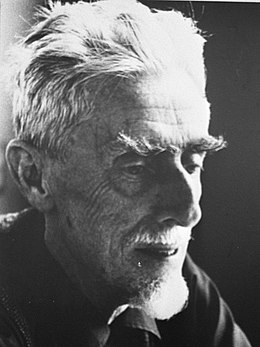
\includegraphics [scale=0.5] {image/escher.jpg}
    \caption{Portrait d'Escher en 1971, 1 an avant son décès}
\end{figure}

\begin{figure} [!h]
    \center
    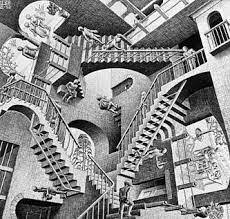
\includegraphics [scale=0.5] {image/dessin1_escherjpg.jpg}
    \caption{Diamants aztèques d'ordre 1, 2, 3 et 6}
\end{figure}

\begin{figure} [!h]
    \center
    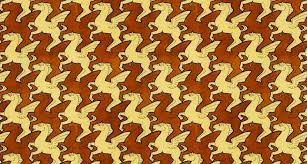
\includegraphics [scale=0.5] {image/dessin2_escherjpg.jpg}
    \caption{Diamants aztèques d'ordre 1, 2, 3 et 6}
\end{figure}

\begin{figure} [!h]
    \center
    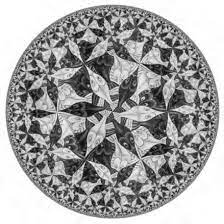
\includegraphics [scale=0.5] {image/dessin3_escher.jpg}
    \caption{Diamants aztèques d'ordre 1, 2, 3 et 6}
\end{figure}

William Thurston: mathématicien américain né en 1946 et mort en 2012, spécialisé dans la topologie sur les espaces bi et tri-dimensionnels et dont il fut recompenser par la médaille Fields en 1983.

\begin{figure} [!h]
    \center
    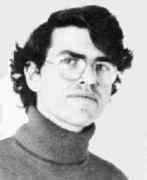
\includegraphics [scale=0.5] {image/thurston.jpg}
    \caption{Portrait de Thurston en 1991}
\end{figure}

Evgraf Fedorov: mathématicien cristallographe russe né en 1853 et mort en 1919 (polytope à developper)

\begin{figure} [!h]
    \center
    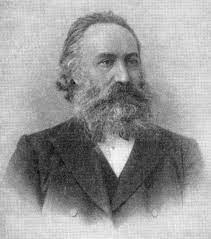
\includegraphics [scale=0.5] {image/Fedorov.jpg}
    \caption{Portrait d'Evgraf Fedorov à la fin du 19eme siècle}
\end{figure}

\nocite{*}
\bibliographystyle{plain}
\bibliography{biblio} % fichier biblio.bib
\end{document}

